% Drawing 154/05-11 -- folder 154, batch 05, archive page 83 (PDF page 84).
% Transcription: au-dessous, deux croquis : un rectangle dont les deux grands côtés portent de petits traits, étiqueté $\nu'$ à gauche et $\nu$ à droite ; un segment joignant deux points, par chacun desquels passe un faisceau de droites, étiquetés $\nu' - 1$ et $\nu - 1$
% Kind: rectangle with ticks; segment between two pencils of lines. Method 2 (schematic redraw from the facsimile). Status: ok.
% Notes: Rectangle: four ticks on the upper long side and four on the lower one, nu' at its left and nu at its right. Segment: a point at each end, five lines through the left one and four through the right one (each pencil through its point), the labels nu' - 1 and nu - 1 above. Redrawn 2026-11-12 (issue 128): to check again.
% Coordinates: 1 unit = 1 mm = 1/100 of the crop width (bbox in page fractions: [0.48, 0.39, 0.76, 0.455]).
% Redrawn by Claude (claude-fable-5-2), issue #128, 2026-11-12; not checked by a human; not compiled (no TeX in the session).
% Rights: reproduces part of the work -- behind RENDER_TRANSCRIPTS, never published by itself.
\documentclass[tikz,border=3pt]{standalone}
\usepackage{amsmath,amssymb}
\usetikzlibrary{patterns,arrows.meta}
\tikzset{pencil/.style={black!45}, struck/.style={black!35}, mpt/.style={circle,draw,inner sep=1.3pt}, pt/.style={circle,fill,inner sep=0.9pt}, opt/.style={circle,draw,fill=white,inner sep=1.1pt}}
\begin{document}
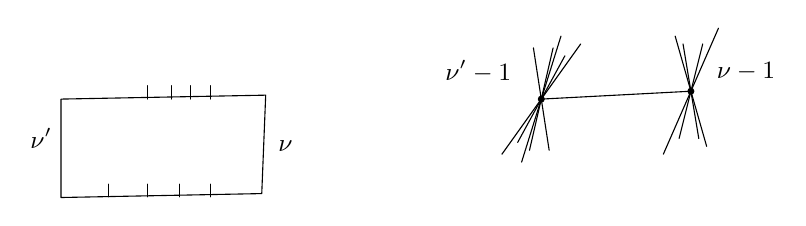
\begin{tikzpicture}[x=1mm,y=1mm,line cap=round,line join=round,font=\scriptsize]
\draw (4,-12) -- (30,-11.5) -- (29.5,-24) -- (4,-24.5) -- cycle;
\draw (15,-10.3) -- (15,-12);
\draw (18,-10.3) -- (18,-12);
\draw (20.5,-10.3) -- (20.5,-12);
\draw (23,-10.3) -- (23,-12);
\draw (10,-22.8) -- (10,-24.4);
\draw (15,-22.8) -- (15,-24.4);
\draw (19,-22.8) -- (19,-24.4);
\draw (23,-22.8) -- (23,-24.4);
\node[inner sep=1pt] at (1.5,-17) {\small $\nu'$};
\node[inner sep=1pt] at (32.5,-18) {\small $\nu$};
\draw (65,-12) -- (84,-11);
\node[pt] at (65,-12) {};
\node[pt] at (84,-11) {};
\draw (60,-19) -- (70,-5);
\draw (62.5,-20) -- (67.5,-4);
\draw (64,-5.5) -- (66,-18.5);
\draw (66.5,-5.5) -- (63.5,-18.5);
\draw (68,-6.5) -- (62,-17.5);
\draw (80.5,-19) -- (87.5,-3);
\draw (83,-5) -- (85,-17);
\draw (85.5,-5) -- (82.5,-17);
\draw (86,-18) -- (82,-4);
\node[inner sep=1pt] at (57,-8.5) {\small $\nu'-1$};
\node[inner sep=1pt] at (91,-8.5) {\small $\nu-1$};
\end{tikzpicture}
\end{document}
